% Provenance (never printed): see sources/outline_sources.md (Year 3: the
% structure of the Galaxy; the rotation curve and dark matter; galaxy types;
% the distance ladder, Hubble's law recalled from the physics books).
% Brief: sources/book5/BRIEFS.md, ch. 29. Curves from figdata/bachelor-3/
% rotation_curve.py (the circular velocity curve of Eilers et al. 2019 with the
% Pouliasis et al. 2017 Model I baryons and an NFW halo fitted to it) and
% distance_ladder.py (the OGLE-IV Cepheids of the Large Magellanic Cloud, CDS
% J/AcA/65/297, and the ranges of the rungs). Exercise and problem values in the
% Book 5 scratch calculator calc/ch29.py. The survey of Part I of the problem and
% the galaxies of the exercises are invented.
\chapter{La Voie lactée et les galaxies}\label{ch:b3:milky-way-galaxies}

Dans le Système solaire, les planètes éloignées du Soleil se déplacent lentement~: Mercure
tourne autour de lui à \qty{47.4}{km.s^{-1}}, Neptune à \qty{5.4}{km.s^{-1}}, comme
l'exige la troisième loi de Kepler pour des corps soumis à une seule masse centrale. Les étoiles
de la Galaxie ne se comportent pas ainsi. Mesurée à partir des mouvements de plus de
vingt mille géantes rouges, la vitesse de leurs orbites circulaires vaut
\qty{227}{km.s^{-1}} à \qty{5}{kpc} du centre, \qty{229}{km.s^{-1}}
au niveau du Soleil, et encore \qty{198}{km.s^{-1}} à \qty{25}{kpc}, là où il ne subsiste
pratiquement plus d'étoiles ni de gaz. Si la masse que nous voyons était tout ce qui existe, les étoiles
périphériques seraient bien plus lentes. Quelque chose d'invisible les retient. Ce chapitre
décrit la Galaxie que nous habitons, en évalue la masse à partir de sa rotation, classe les
autres galaxies en types, et gravit la chaîne de méthodes par lesquelles on mesure leurs
distances, ainsi que l'expansion de l'Univers.
% ledger: planet:Mercury.vorb, planet:Neptune.vorb, eilers19:vc, eilers19:table1

\begin{recall}
La Voie lactée, l'effet Doppler, les lois de Kepler, le théorème de Newton sur l'attraction
d'une coquille sphérique, la matière noire, les trous noirs et leur rayon de Schwarzschild, les
supernovæ, les naines blanches, la raie à \qty{21}{cm} de l'hydrogène atomique et la loi de
Hubble sont traités dans les volumes de physique. La parallaxe annuelle, le parsec, le flux et la
luminosité, les magnitudes apparente et absolue, le module de distance, les bandes
photométriques et l'indice de couleur figurent dans le volume de première année, au chapitre
consacré aux télescopes et à la photométrie. Le milieu interstellaire et ses poussières sont
traités dans le volume de deuxième année, au chapitre consacré au milieu interstellaire et à la
formation stellaire.
\end{recall}

\section{La structure de la Galaxie}\label{sec:b3:milky-way-galaxies:structure}

Vue depuis la Terre, la Galaxie est la Voie lactée~: une bande de lumière qui fait le tour
du ciel, traversée de sombres traînées de poussière et plus brillante en direction de la
constellation du Sagittaire, où se trouve son centre. Cette bande est le disque dans lequel
se situe le Soleil, vu par la tranche depuis l'intérieur.

\begin{omfigure}
\centering
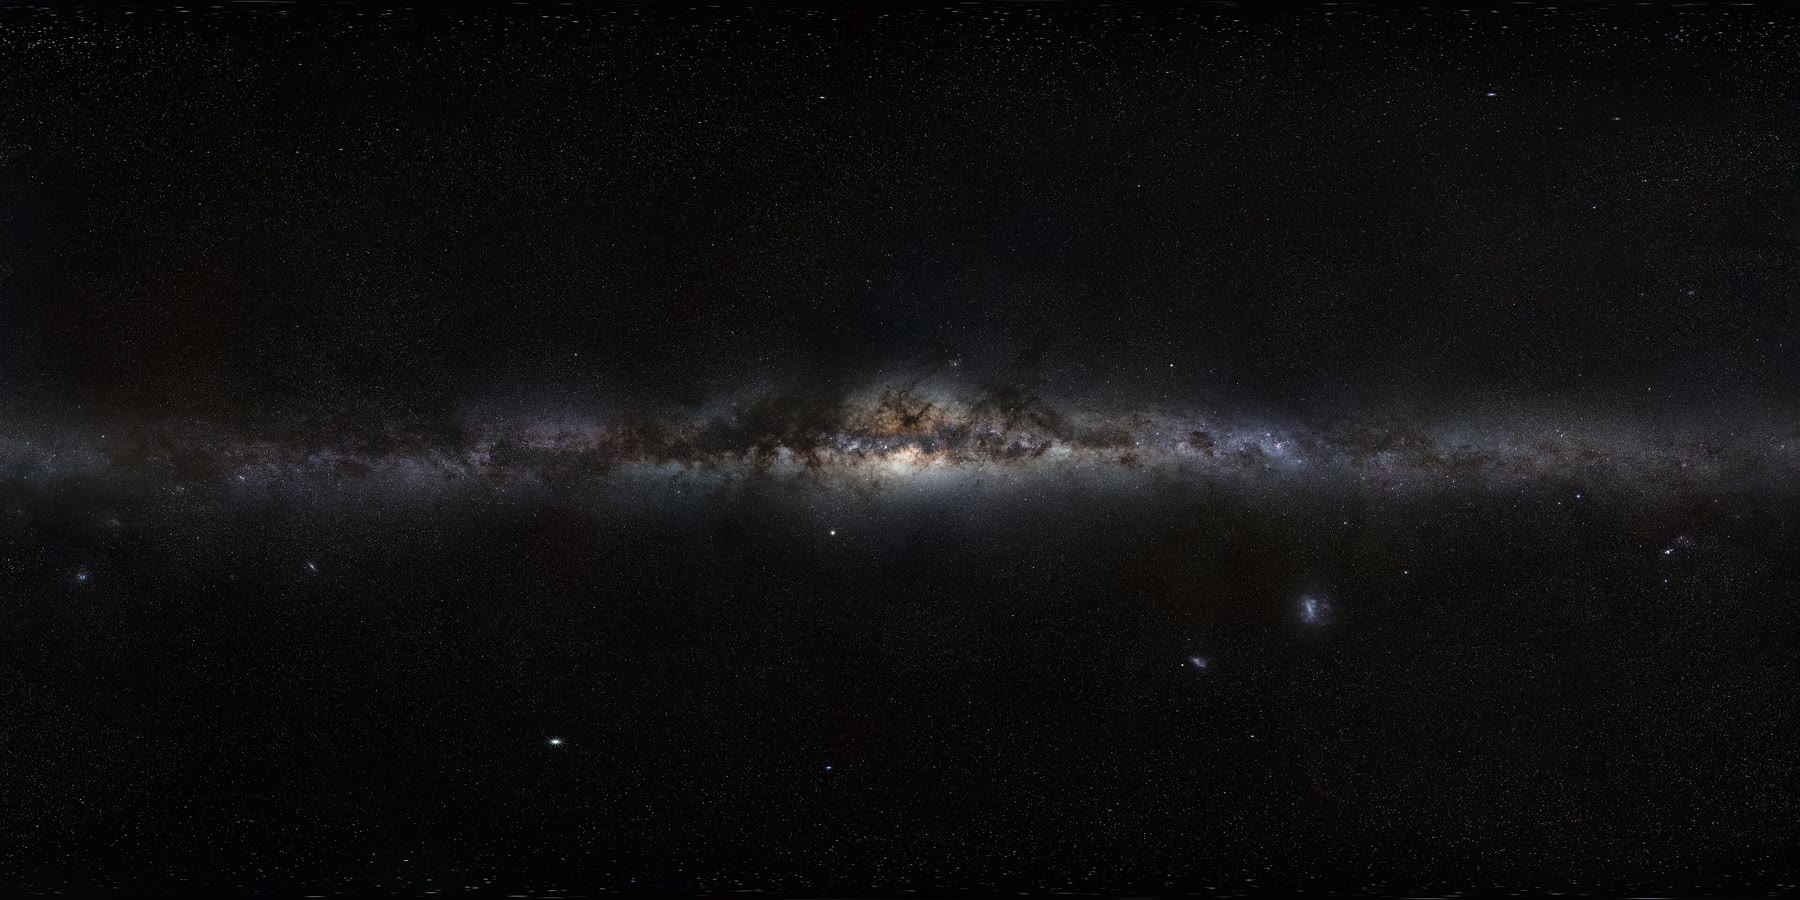
\includegraphics[width=0.96\linewidth]{images/book5/b3-milky-way-panorama.jpg}
\par\smallskip{\small Le ciel entier en une seule image, projeté de sorte que le
plan de la Galaxie traverse le milieu et que son centre se trouve au
centre de l'image. La bande est le disque vu de l'intérieur~; les sombres
traînées sont la poussière du disque, qui masque les étoiles situées derrière elle~;
le bulbe central se gonfle autour du centre. Les deux petites taches sous la bande, à
droite, sont le Grand et le Petit Nuage de Magellan, deux galaxies satellites~;
la faible tache sous la bande, près du bord gauche, est la galaxie d'Andromède.
Photographie ESO/S.~Brunier, CC BY~4.0.}\label{fig:b3:milky-way-galaxies:panorama}
\end{omfigure}
% ledger: photo:b3-milky-way-panorama, mcconn12:local-group

\begin{definition}[Disque galactique, disque épais, bulbe galactique et halo stellaire]\label{def:b3:milky-way-galaxies:structure}
Le \emph{disque galactique}\index{disque galactique} est la composante aplatie de
la Galaxie, formée d'étoiles, de gaz et de poussières en orbites presque circulaires autour de son
centre~; sa densité décroît à peu près exponentiellement avec la hauteur au-dessus de son
plan médian et avec la distance au centre, sur une hauteur d'échelle et une longueur d'échelle.
Le \emph{disque épais}\index{disque épais} est une seconde composante de disque, plus ancienne,
de hauteur d'échelle plus grande et de masse plus faible. Le
\emph{bulbe galactique}\index{bulbe galactique} est la concentration centrale d'étoiles qui
se gonfle au-dessus du disque. Le \emph{halo stellaire}\index{halo stellaire}
est la composante clairsemée, à peu près sphéroïdale, formée d'étoiles âgées et d'amas
globulaires, qui entoure le disque et le bulbe.
\end{definition}

La Galaxie est une spirale barrée. Au voisinage du Soleil, le disque mince a une
hauteur d'échelle d'environ \qty{300}{pc} et le \omterm{def:b3:milky-way-galaxies:structure}{disque épais} d'environ
\qty{900}{pc}~; leurs longueurs d'échelle valent environ \qty{2.6}{kpc} et
\qty{2.0}{kpc}. Le \omterm{def:b3:milky-way-galaxies:structure}{disque épais} renferme quelque \num{6e9} masses solaires,
soit à peu près un cinquième du disque mince. Vu de côté, le bulbe a la forme
d'une boîte ou d'une cacahuète~: c'est la partie intérieure épaissie d'une barre
d'étoiles de \qty{5}{kpc} de demi-longueur, dont l'axe long fait un angle de
\ang{27} avec la droite qui joint le Soleil au centre. Le \omterm{def:b3:milky-way-galaxies:structure}{halo stellaire} ne renferme
qu'environ un pour cent des étoiles. Au total, les étoiles de la Galaxie
pèsent environ \num{5e10} masses solaires.
% ledger: bhg16:structure

\begin{omfigure}
\centering
\begin{tikzpicture}[x=0.17cm, y=0.17cm, font=\scriptsize]
% edge-on view
\begin{scope}
\fill[omProp!8] (0,0) circle (17);
\draw[omProp!60, densely dotted] (0,0) circle (17);
\fill[black!12] (0,0) ellipse (15 and 2.4);
\fill[black!30] (0,0) ellipse (15 and 0.8);
\fill[black!45] (-3.2,0) .. controls (-3.4,2.3) and (-1.2,2.0) .. (0,1.4)
  .. controls (1.2,2.0) and (3.4,2.3) .. (3.2,0)
  .. controls (3.4,-2.3) and (1.2,-2.0) .. (0,-1.4)
  .. controls (-1.2,-2.0) and (-3.4,-2.3) .. (-3.2,0) -- cycle;
\foreach \p in {(-10,9),(6,12),(12,-7),(-6,-13),(-13,-4),(3,-9),(12,8)}
  \fill[omProp] \p circle (0.35);
\fill[ocYellow, draw=black] (-8.2,0.15) circle (0.55);
\node[anchor=south] at (-8.2,0.9) {Soleil};
\draw[|<->|] (0,-4.6) -- node[below] {$R_0 \approx \qty{8.2}{kpc}$} (-8.2,-4.6);
\node[anchor=west] at (15.3,0) {disque mince};
\node[anchor=west] at (13.2,2.8) {disque épais};
\draw[->] (4.6,4.6) node[anchor=south west, inner sep=1pt] {bulbe} -- (2.4,1.7);
\node[omProp!80!black] at (-11,13.5) {halo stellaire};
\node at (0,-19.5) {(a) vue par la tranche};
\end{scope}
% face-on view
\begin{scope}[xshift=7.6cm]
\fill[omProp!8] (0,0) circle (17);
\draw[omProp!60, densely dotted] (0,0) circle (17);
\fill[black!12] (0,0) circle (15);
\foreach \a in {0,180} {
  \draw[line width=1.6pt, black!40, rotate=\a+63]
    plot[domain=0:3.9, samples=50] ({5*exp(0.25*\x)*cos(\x r)}, {5*exp(0.25*\x)*sin(\x r)});
}
\fill[black!45, rotate=63] (0,0) ellipse (5 and 1.5);
\draw[dashed] (0,0) circle (8.2);
\fill[ocYellow, draw=black] (0,-8.2) circle (0.55);
\node[anchor=north] at (0,-8.9) {Soleil};
\draw[dotted, thick] (0,0) -- (0,-8.2);
\draw[thick, ->] (0,0) ++(25:16) arc (25:-25:16);
\node[anchor=west] at (17.3,0) {rotation};
\node[anchor=west, fill=black!12, inner sep=1pt] at (3.4,3.4) {barre};
\draw[|-|] (6,-15.5) -- node[below] {\qty{5}{kpc}} (11,-15.5);
\node at (0,-19.5) {(b) vue depuis le pôle galactique nord};
\end{scope}
\end{tikzpicture}
\par\smallskip{\small Esquisse de la Galaxie, à l'échelle pour ses principales
dimensions. (a)~Vue par la tranche~: le disque mince (bande sombre), le \omterm{def:b3:milky-way-galaxies:structure}{disque épais} (bande
claire), le bulbe en forme de boîte et le \omterm{def:b3:milky-way-galaxies:structure}{halo stellaire} avec ses amas globulaires (points
orangés)~; le Soleil se trouve dans le disque, à environ \qty{8.2}{kpc}
du centre et à environ \qty{25}{pc} au-dessus du plan médian (trop petit pour
être représenté). (b)~Vue depuis le pôle galactique nord~: la barre, de
\qty{5}{kpc} de demi-longueur, inclinée de \ang{27} par rapport à la droite joignant le Soleil
au centre (pointillés)~; le cercle solaire (tirets)~; les bras spiraux
dessinés de façon schématique~; la Galaxie tourne dans le sens horaire sur cette vue.}\label{fig:b3:milky-way-galaxies:sketch}
\end{omfigure}
% ledger: bhg16:structure, gravity19:r0

\begin{definition}[Population stellaire]\label{def:b3:milky-way-galaxies:populations}
Une \emph{population stellaire}\index{population stellaire} est un groupe d'étoiles
d'une galaxie qui partagent une plage d'âges, de compositions chimiques et de
orbites. Les jeunes étoiles du disque mince, riches en éléments plus lourds que
l'hélium et sur des orbites presque circulaires, sont traditionnellement appelées
population~I~; les vieilles étoiles du halo et des amas globulaires, pauvres
en éléments lourds et sur des orbites à grands mouvements aléatoires avec peu de
rotation nette, population~II.
\end{definition}

Le \omterm{def:b3:milky-way-galaxies:structure}{disque épais} occupe une position intermédiaire~: ses étoiles sont en majorité
plus âgées que celles du disque mince et, à teneur en fer donnée, plus riches en
éléments légers que les astronomes appellent éléments alpha, mesurés par rapport au fer. Le
\omterm{def:b3:milky-way-galaxies:structure}{halo stellaire} est un
enregistrement fossile~: une grande partie de celui-ci a été assemblée à partir de petites galaxies tombées dans
la Galaxie et déchirées par ses marées, et certains de leurs courants d'étoiles
peuvent encore être suivis à travers le ciel.
% ledger: bhg16:populations

\begin{definition}[Coordonnées galactiques]\label{def:b3:milky-way-galaxies:coordinates}
Les \emph{coordonnées galactiques}\index{coordonnées galactiques} d'une direction
sont sa \emph{latitude galactique} $b$, l'angle par rapport au plan galactique
(positif vers le pôle galactique nord), et sa \emph{longitude
galactique} $\ell$, mesurée dans le plan à partir de la direction du centre
galactique ($\ell = 0$) jusqu'à $\ell = \ang{90}$, la direction vers laquelle
la rotation de la Galaxie entraîne le Soleil. Le plan a été défini en 1958 comme
le plan principal de l'hydrogène atomique de la Galaxie~;
le pôle galactique nord se situe à une ascension droite de \ang{192.25}
($12^\mathrm{h}49^\mathrm{m}$) et une déclinaison de \ang{27.4} (équinoxe
1950).
\end{definition}
% ledger: liu11:galactic, reid20:sgra

Le Soleil n'est pas tout à fait dans le plan~: il se trouve à environ \qty{25}{pc} au nord de celui-ci.
Sa distance au centre, $R_0$, a longtemps été la grandeur la plus incertaine de
l'astronomie galactique. Elle est désormais mesurée géométriquement~: l'étoile S2
tourne autour du trou noir central de la Galaxie sur une orbite de \num{16} ans,
dont la taille angulaire sur le ciel et la vitesse le long de la ligne de visée,
suivies pendant 27 ans, donnent directement la distance au centre~:
$R_0 = \qty{8178}{pc}$, avec une erreur statistique de \qty{13}{pc} et une
erreur systématique de \qty{22}{pc}. Une revue de toutes les méthodes donne
$R_0 = \qty[separate-uncertainty=true]{8.2 \pm 0.1}{kpc}$.
% ledger: bhg16:structure, gravity19:r0

\section{Rotation et halo sombre}\label{sec:b3:milky-way-galaxies:rotation}

\begin{definition}[Référentiel local au repos]\label{def:b3:milky-way-galaxies:lsr}
Le \emph{référentiel local au repos}\index{référentiel local au repos} (LSR) est
le référentiel qui se déplace sur l'orbite circulaire autour du centre galactique
passant par la position actuelle du Soleil. Les vitesses des étoiles et du gaz
proches y sont rapportées.
\end{definition}

Le Soleil se déplace par rapport au LSR d'environ \qty{10}{km.s^{-1}} en direction du
centre galactique, de \qty{11}{km.s^{-1}} dans le sens de la rotation et de
\qty{7}{km.s^{-1}} vers le pôle galactique nord~: un petit mouvement propre
qui s'ajoute à une orbite de vitesse $V_0$ de quelques centaines de kilomètres
par seconde. Vue depuis la Terre, la source radio au centre de la Galaxie dérive
le long du plan galactique de \qty{6.411}{mas} par an~; presque toute cette
dérive est le reflet de l'orbite du Soleil, et elle donne la vitesse totale du
Soleil autour du centre, \qty[separate-uncertainty=true]{248 \pm 3}{km.s^{-1}}
(\cref{exo:b3:milky-way-galaxies:2}).
% ledger: bhg16:lsr, reid20:sgra

\begin{definition}[Courbe de rotation~; constantes d'Oort]\label{def:b3:milky-way-galaxies:rotation-curve}
La \emph{courbe de rotation}\index{courbe de rotation} d'une galaxie à disque est la
vitesse $V(R)$ d'une orbite circulaire dans son plan en fonction de la
distance $R$ à son centre. Pour la Galaxie, avec $V_0 = V(R_0)$ et
$V'_0 = \mathrm{d}V/\mathrm{d}R$ en $R_0$, les \emph{constantes
d'Oort}\index{constantes d'Oort} sont
\[
A = \frac12\left(\frac{V_0}{R_0} - V'_0\right), \qquad
B = -\frac12\left(\frac{V_0}{R_0} + V'_0\right).
\]
\end{definition}

$A$ mesure le cisaillement de la rotation du disque et $B$ sa vorticité~: dans un
disque tournant comme un corps solide, $V'_0 = V_0/R_0$ et $A = 0$~; pour une \omterm{def:b3:milky-way-galaxies:rotation-curve}{courbe
de rotation} plate, $A = -B$. Leur différence est la vitesse angulaire du LSR,
$A - B = V_0/R_0 = \omega_0$, et leur somme la pente, $A + B = -V'_0$.

\begin{theorem}[Formules d'Oort]\label{thm:b3:milky-way-galaxies:oort}
Une étoile située à une distance $d \ll R_0$ du Soleil, dans le plan galactique à la
longitude $\ell$, sur une orbite circulaire, possède par rapport au LSR la vitesse radiale
$v_r$ et la vitesse transverse $v_t$ (positive dans le sens des $\ell$
croissants)
\[
v_r = A\,d\sin 2\ell, \qquad v_t = d\,(A\cos 2\ell + B),
\]
au premier ordre en $d/R_0$.
\end{theorem}

\begin{proof}
Soit $\omega(R) = V(R)/R$ la vitesse angulaire de l'orbite en $R$. Plaçons
le centre galactique à l'origine, le Soleil à la distance $R_0$, et soit l'étoile à la
distance $R$ du centre, sa position vue depuis le centre faisant l'angle $\theta$ avec
celle du Soleil. En projetant la vitesse de l'étoile $\omega R$ et la vitesse du LSR
$\omega_0 R_0$ sur la ligne de visée, un peu de trigonométrie dans le triangle
Soleil--étoile--centre (la loi des sinus donne $R\sin(\ell + \theta) = R_0\sin\ell$)
donne le résultat exact $v_r = R_0\,[\omega(R) - \omega_0]\sin\ell$.
De même, sur la direction
perpendiculaire à la ligne de visée,
$v_t = R_0\,[\omega(R) - \omega_0]\cos\ell - \omega(R)\,d$. Pour une
étoile proche, $\omega(R) - \omega_0 \approx \omega'_0\,(R - R_0)$ et
$R - R_0 \approx -d\cos\ell$. Alors
$v_r \approx -R_0\omega'_0\,d\cos\ell\sin\ell = -\tfrac12 R_0\omega'_0\,
d\sin 2\ell$ et, en gardant les termes du premier ordre,
$v_t \approx -R_0\omega'_0\,d\cos^2\ell - \omega_0 d$. Avec
$\omega'_0 = V'_0/R_0 - V_0/R_0^2$, $-\tfrac12 R_0\omega'_0 = A$ et
$-R_0\omega'_0\cos^2\ell - \omega_0 = A(1 + \cos 2\ell) - (A - B) =
A\cos 2\ell + B$.
\end{proof}

Les vitesses radiales des étoiles proches varient donc comme $\sin 2\ell$ sur
la voûte céleste, et leurs mouvements propres comme $\cos 2\ell$ autour d'une moyenne fixée par $B$.
D'après les mouvements propres et les parallaxes de \num{304267} étoiles du premier
catalogue Gaia, à une distance typique de \qty{230}{pc}, les \omterm{def:b3:milky-way-galaxies:rotation-curve}{constantes d'Oort}
sont $A = \qty[separate-uncertainty=true]{15.3 \pm 0.4}{km.s^{-1}.kpc^{-1}}$
et $B = \qty[separate-uncertainty=true]{-11.9 \pm 0.4}{km.s^{-1}.kpc^{-1}}$.
Deux termes supplémentaires qu'un disque axisymétrique n'aurait pas,
appelés $C$ et $K$, ressortent à environ \qty{-3}{km.s^{-1}.kpc^{-1}}~:
le disque local est brassé par la barre et les bras spiraux.
% ledger: bovy17:oort

\subsection*{La courbe de rotation à partir de la raie à 21~cm}

L'hydrogène atomique remplit le disque et émet la raie à 21~cm, à
\qty{1420.405751}{MHz}~; les ondes radio traversent la poussière qui masque le
disque lointain aux longueurs d'onde visibles. Le long d'une ligne de visée
dans le plan, chaque nuage de gaz ajoute sa raie au décalage Doppler de
sa vitesse radiale, et le profil de la raie est un spectre de
vitesses. À l'intérieur du cercle solaire, une vitesse se détache.
% ledger: nrao:hi-line

\begin{theorem}[Méthode du point de tangence]\label{thm:b3:milky-way-galaxies:tangent}
Supposons que le gaz décrive des orbites circulaires de vitesse angulaire $\omega(R)$
décroissante vers l'extérieur. Le long d'une ligne de visée de longitude
$0 < \ell < \ang{90}$, la vitesse radiale par rapport au \omterm{def:b3:milky-way-galaxies:lsr}{référentiel local au repos} est maximale
au point de tangence, où la ligne de visée est tangente à une orbite, en
$R = R_0\sin\ell$, et sa valeur maximale vaut
\[
v_\mathrm{max} = V(R_0\sin\ell) - V_0\sin\ell .
\]
\end{theorem}

\begin{proof}
D'après la démonstration des formules d'Oort, le gaz situé à la distance $R$ du centre sur
la ligne de visée a $v_r = R_0\,[\omega(R) - \omega_0]\sin\ell$. Avec
$\sin\ell > 0$ et $\omega$ décroissante, $v_r$ est maximale là où $R$ est
minimal. Le long de la ligne de visée, $R$ est minimal au pied de la
perpendiculaire issue du centre, où $R = R_0\sin\ell$. Là,
$R_0\,\omega(R)\sin\ell = \omega(R)\,R = V(R)$ et
$R_0\,\omega_0\sin\ell = V_0\sin\ell$.
\end{proof}

\begin{omfigure}
\centering
\begin{tikzpicture}[scale=0.95, font=\small]
\coordinate (C) at (0,0);
\coordinate (S) at (0,-4);
\coordinate (T) at (-1.970,-1.653);
\draw[dashed, black!50] (C) circle (4);
\draw[dashed, omDef!70] (C) circle (2.571);
\fill (C) circle (2pt) node[anchor=south west] {Centre galactique};
\fill[ocYellow, draw=black] (S) circle (3pt);
\node[anchor=north] at (0,-4.15) {Soleil};
\draw[thick] (S) -- ($(S)!2.25!(T)$) node[anchor=south east, fill=white, inner sep=1pt] {ligne de visée};
\draw[dotted, thick] (C) -- (S);
\draw[thick, omThm] (C) -- node[anchor=north west, fill=white, inner sep=1pt, pos=0.45] {$R_0\sin\ell$} (T);
\fill[omThm] (T) circle (2pt);
\node[anchor=north east, omThm, fill=white, inner sep=1pt] at ($(T)+(-0.05,-0.08)$) {point de tangence};
\draw[->, very thick, omDef] (T) -- ++(-0.643*1.3, 0.766*1.3) node[anchor=south west, fill=white, inner sep=1pt] {$V(R)$};
\draw[->, very thick, black!70] (S) -- ++(-1.4,0) node[anchor=north] {$V_0$};
\draw (0,-3.2) arc (90:130:0.8);
\node at (-0.30,-2.85) {$\ell$};
\node[anchor=west] at (0.1,-2.2) {$R_0$};
\node[black!60, anchor=west] at (2.9,-2.9) {cercle solaire};
\end{tikzpicture}
\par\smallskip{\small La méthode du point de tangence, vue depuis le pôle
galactique nord. Le long d'une ligne de visée de longitude $\ell$, le gaz le plus
proche du centre se trouve au point de tangence, à $R = R_0\sin\ell$ (en rouge)~; sa
vitesse orbitale $V(R)$ est dirigée le long de la ligne de visée, et la
vitesse radiale y est la plus grande que montre le profil de la raie.
Chaque longitude donne un point de la \omterm{def:b3:milky-way-galaxies:rotation-curve}{courbe de rotation} à l'intérieur du cercle solaire.}\label{fig:b3:milky-way-galaxies:tangent}
\end{omfigure}

La vitesse la plus élevée de chaque profil à 21~cm donne donc $V$ en
$R_0\sin\ell$, et un balayage des longitudes de \ang{0} à \ang{90} donne
la \omterm{def:b3:milky-way-galaxies:rotation-curve}{courbe de rotation} depuis le centre jusqu'au Soleil. Au-delà du
cercle solaire, aucune ligne de visée n'est tangente à une orbite et la
méthode échoue~: il faut alors mesurer la distance de chaque traceur en plus
de sa vitesse. Depuis 2014, un satellite a mesuré les parallaxes de plus
d'un milliard d'étoiles, et la \omterm{def:b3:milky-way-galaxies:rotation-curve}{courbe de rotation} externe est désormais tracée par des étoiles.
% ledger: nrao:hi-line, gaia:dr3

\begin{omfigure}
\centering
\begin{tikzpicture}
\begin{axis}[width=0.90\linewidth, height=0.52\linewidth,
  xmin=0, xmax=26, ymin=0, ymax=265,
  xlabel={distance au centre galactique $R$ (kpc)}, ylabel={vitesse circulaire (\unit{km.s^{-1}})},
  tick label style={font=\scriptsize}, label style={font=\small},
  legend style={font=\scriptsize, at={(0.5,-0.16)}, anchor=north, legend columns=4, draw=none, cells={anchor=west}, /tikz/every even column/.append style={column sep=1em}}]
\addplot[thin, black!40, dashed, forget plot] coordinates {(8.122,0) (8.122,265)};
\node[font=\scriptsize, anchor=south west, rotate=90] at (axis cs:7.9,4) {Soleil};
\addplot[only marks, mark=*, mark size=1.1pt, black, error bars/.cd, y dir=both, y explicit]
  table[x=R, y=vc, y error minus=sig_lo, y error plus=sig_hi] {figdata/out/bachelor-3-rotation_curve-data.dat};
\addlegendentry{mesuré}
\addplot[very thick, omDef] table[x=R, y=v_tot] {figdata/out/bachelor-3-rotation_curve-model.dat};
\addlegendentry{modèle total}
\addplot[thick, black!55] table[x=R, y=v_bar] {figdata/out/bachelor-3-rotation_curve-model.dat};
\addlegendentry{ensemble des baryons}
\addplot[thick, dashed, red!70!black] table[x=R, y=v_halo] {figdata/out/bachelor-3-rotation_curve-model.dat};
\addlegendentry{halo de matière noire}
\addplot[densely dotted, thick, omProp] table[x=R, y=v_bulge] {figdata/out/bachelor-3-rotation_curve-model.dat};
\addlegendentry{bulbe}
\addplot[dashdotted, thick, omMeth] table[x=R, y=v_thin] {figdata/out/bachelor-3-rotation_curve-model.dat};
\addlegendentry{disque mince}
\addplot[densely dashed, thick, violet!70!black] table[x=R, y=v_thick] {figdata/out/bachelor-3-rotation_curve-model.dat};
\addlegendentry{disque épais}
\end{axis}
\end{tikzpicture}
\par\smallskip{\small La \omterm{def:b3:milky-way-galaxies:rotation-curve}{courbe de rotation} de la Galaxie. Points~: la vitesse circulaire
mesurée à partir des géantes rouges entre 5 et \qty{25}{kpc} (Eilers
et al., 2019), avec ses barres d'erreur. Courbes~: les vitesses que
donneraient seuls le bulbe, le disque mince et le \omterm{def:b3:milky-way-galaxies:structure}{disque épais} d'un modèle
de masse publié (Pouliasis et al., 2017), leur combinaison (en gris), et
le \omterm{def:b3:milky-way-galaxies:halo}{halo de matière noire} ajusté ici aux mesures (tirets rouges), qui prend
le relais des baryons au-delà de \qty{14}{kpc}~; ils s'ajoutent en quadrature au
total (en bleu). Les \qty{5}{kpc} intérieurs, où la barre rend les orbites
nettement non circulaires, sont exclus de la mesure.}\label{fig:b3:milky-way-galaxies:rotation}
\end{omfigure}
% ledger: eilers19:table1, eilers19:vc, eilers19:halo, pouliasis17:model1, data:b5-rotation-fit

La courbe de la figure ci-dessus a été mesurée à partir des positions, des distances
et des vitesses de plus de vingt-trois mille géantes rouges lumineuses,
à l'aide de l'équation de l'hydrodynamique stellaire qui relie les mouvements
moyens d'une population d'étoiles à la gravité qui les retient (l'équation de Jeans).
Au niveau du Soleil, elle donne $V_0 = \qty{229.0}{km.s^{-1}}$, avec une
incertitude systématique de deux à cinq pour cent~; au-delà, elle décroît lentement,
de \qty[separate-uncertainty=true]{1.7 \pm 0.1}{km.s^{-1}} par kiloparsec. Elle
ne décroît pas comme l'exigerait la masse visible.
% ledger: eilers19:vc

\subsection*{Peser la Galaxie}

La gravité d'un disque n'est pas celle d'une sphère, mais la courbe des vitesses d'un
modèle de masse se calcule aisément lorsque chaque composante possède un potentiel
sous forme close. Les potentiels dans le plan ci-dessous sont ceux d'un modèle publié
des étoiles de la Galaxie.

\begin{proposition}[Vitesses circulaires de trois modèles de masse]\label{prop:b3:milky-way-galaxies:models}
Dans le plan $z = 0$, la vitesse circulaire $V^2 = R\,\partial\Phi/\partial R$
vaut, pour
\begin{itemize}
\item une sphère de Plummer de masse $M$ et de rayon de cœur $b$, de potentiel
  $\Phi = -GM/\sqrt{r^2 + b^2}$~:
  \[ V^2 = \frac{GMR^2}{(R^2 + b^2)^{3/2}}\,; \]
\item un disque de Miyamoto--Nagai de masse $M$, de longueur d'échelle $a$ et de
  hauteur d'échelle $b$, de potentiel
  $\Phi = -GM\big/\sqrt{R^2 + \bigl(a + \sqrt{z^2 + b^2}\,\bigr)^2}$~:
  \[ V^2 = \frac{GMR^2}{\bigl(R^2 + (a + b)^2\bigr)^{3/2}}\,; \]
\item un halo de Navarro--Frenk--White de densité
  $\rho = \rho_0\big/\bigl[x(1 + x)^2\bigr]$, $x = r/R_s$~: la masse à l'intérieur de $r$
  vaut $M(r) = 4\pi\rho_0R_s^3\bigl[\ln(1 + x) - x/(1 + x)\bigr]$ et
  $V^2 = GM(r)/r$.
\end{itemize}
Pour plusieurs composantes, les carrés des vitesses s'ajoutent.
\end{proposition}

\begin{proof}
Pour les deux premiers, on dérive le potentiel par rapport à $R$ en
$z = 0$. Pour le halo, on intègre $4\pi r^2\rho$ de 0 à $r$~: avec
$u = 1 + x'$, $\int_0^x x'\,\mathrm{d}x'/(1 + x')^2 =
\int_1^{1+x}(u - 1)\,\mathrm{d}u/u^2 = \ln(1 + x) + 1/(1 + x) - 1$~; une
masse sphérique agit sur une orbite à $r$ comme si toute sa masse située à
l'intérieur de $r$ était au centre (théorème de Newton). Les potentiels
s'ajoutent, d'où leurs dérivées radiales.
\end{proof}

Le modèle utilisé dans la figure comporte un bulbe de Plummer de
\num{1.07e10} masses solaires avec $b = \qty{0.3}{kpc}$, un disque mince et un
\omterm{def:b3:milky-way-galaxies:structure}{disque épais} de \num{3.94e10} masses solaires chacun, avec $(a, b) =
(\qty{5.3}{kpc}, \qty{0.25}{kpc})$ et $(\qty{2.6}{kpc}, \qty{0.8}{kpc})$.
Avec $G = \qty{4.301e-6}{kpc.(km.s^{-1})^2}$ par masse solaire, ses étoiles
seules donneraient au Soleil une vitesse orbitale de \qty{184}{km.s^{-1}}, et une
étoile à \qty{20}{kpc} une vitesse de \qty{134}{km.s^{-1}}~; les vitesses mesurées
valent 229 et \qty{200}{km.s^{-1}}. Un halo ajusté aux mesures, les étoiles étant
maintenues fixes, a $R_s = \qty{14.75}{kpc}$ et
$\rho_0 = \num{1.06e7}$ masses solaires par kiloparsec cube, soit la même valeur que
le halo ajusté par ses auteurs ($R_s = \qty[separate-uncertainty=true]{14.8 \pm 0.4}{kpc}$,
$\rho_0 = \qty[separate-uncertainty=true]{1.06 \pm 0.09 e7}{}$ masses solaires
par kiloparsec cube). Le halo domine au-delà d'environ \qty{14}{kpc}.
% ledger: pouliasis17:model1, data:b5-rotation-fit, eilers19:halo, eilers19:table1, const:G, sun:mass, iau:parsec

\begin{definition}[Halo de matière noire]\label{def:b3:milky-way-galaxies:halo}
Le \emph{halo de matière noire}\index{halo de matière noire} d'une galaxie est la
distribution de matière noire, à peu près sphérique, dans laquelle baignent ses étoiles
et son gaz, bien plus étendue et plus massive que ses composantes visibles, et dont
l'existence se déduit de sa gravité~: de la \omterm{def:b3:milky-way-galaxies:rotation-curve}{courbe de rotation}, des mouvements
des galaxies satellites et des étoiles du halo, et de la déviation de la lumière.
\end{definition}

\begin{theorem}[Masse à l'intérieur d'un rayon]\label{thm:b3:milky-way-galaxies:enclosed}
Pour une distribution sphérique de masse, la vitesse circulaire au rayon $r$
donne la masse qui s'y trouve, $M(r) = rV^2/G$. Une \omterm{def:b3:milky-way-galaxies:rotation-curve}{courbe de rotation} plate,
$V = $ constante, implique $M(r) \propto r$ et une densité
$\rho(r) = V^2/(4\pi G r^2)$.
\end{theorem}

\begin{proof}
Par le théorème de Newton, la gravité en $r$ vaut $GM(r)/r^2$, et elle fournit
l'accélération centripète $V^2/r$ d'une orbite circulaire. Si $V$ est constant,
$\mathrm{d}M/\mathrm{d}r = V^2/G = 4\pi r^2\rho$.
\end{proof}

Pour les disques aplatis, $rV^2/G$ n'est pas exactement la masse située à l'intérieur de $r$, mais
c'est la masse qu'une sphère devrait posséder pour produire la même orbite, et on
l'utilise ici, comme il est courant de le faire, comme masse \emph{dynamique}. La figure ci-dessous
la compare pour les étoiles et pour l'ensemble de la Galaxie.

\begin{omfigure}
\centering
\begin{tikzpicture}
\begin{axis}[width=0.80\linewidth, height=0.50\linewidth,
  xmin=0, xmax=30, ymin=0, ymax=28,
  xlabel={rayon $R$ (kpc)}, ylabel={$RV^2/G$ ($10^{10}$ masses solaires)},
  tick label style={font=\scriptsize}, label style={font=\small},
  legend style={font=\scriptsize, at={(0.03,0.97)}, anchor=north west, draw=none, fill=white, cells={anchor=west}}]
\addplot[very thick, omDef] table[x=R, y=m_tot] {figdata/out/bachelor-3-rotation_curve-mass.dat};
\addlegendentry{total, modèle}
\addplot[only marks, mark=*, mark size=1.1pt, black] table[x=R, y=m_dyn] {figdata/out/bachelor-3-rotation_curve-mdata.dat};
\addlegendentry{total, à partir des vitesses mesurées}
\addplot[thick, black!55] table[x=R, y=m_bar] {figdata/out/bachelor-3-rotation_curve-mass.dat};
\addlegendentry{étoiles, modèle}
\end{axis}
\end{tikzpicture}
\par\smallskip{\small La masse dynamique $RV^2/G$ à l'intérieur du rayon $R$. La
masse visible plafonne vers $9\times10^{10}$ masses solaires, soit la masse
du bulbe et des disques du modèle~; le total continue de croître presque
proportionnellement à $R$, comme l'exige une \omterm{def:b3:milky-way-galaxies:rotation-curve}{courbe de rotation} plate. À
\qty{20}{kpc}, le total est plus de deux fois supérieur à la masse visible.}\label{fig:b3:milky-way-galaxies:mass}
\end{omfigure}
% ledger: data:b5-rotation-fit, eilers19:table1, pouliasis17:model1

Jusqu'où s'étend le halo, et combien il pèse au total, la \omterm{def:b3:milky-way-galaxies:rotation-curve}{courbe de rotation}
du disque ne permet pas de le dire. Extrapolé avec son profil ajusté jusqu'à
son rayon viriel, d'environ \qty{190}{kpc}, le halo ajusté par les auteurs
de la mesure contient environ \num{7e11} masses solaires~; une revue d'autres
estimations donne \num{1.3e12}, dont les baryons ne forment que
sept pour cent. La matière noire au voisinage du Soleil est peu dense~:
environ \qty{0.30}{GeV} d'énergie de masse par centimètre cube, soit un tiers de la masse
d'un proton, ce qui explique qu'elle ne se manifeste que par sa gravité accumulée.
% ledger: eilers19:halo, bhg16:structure, nist:mp

\section{Galaxies}\label{sec:b3:milky-way-galaxies:galaxies}

\begin{definition}[Séquence de Hubble~; galaxies elliptiques, lenticulaires, spirales et irrégulières]\label{def:b3:milky-way-galaxies:types}
La \emph{séquence de Hubble}\index{séquence de Hubble} classe les galaxies d'après
leur apparence. Une \emph{galaxie elliptique}\index{galaxie elliptique}
(type E) est un système d'étoiles lisse, dont la brillance décroît régulièrement
depuis le centre, et sans disque~; elle est notée E$n$, avec $n = 10(1 - b/a)$
et $b/a$ le rapport apparent des axes, de E0 (rond) à E7. Une
\emph{galaxie spirale}\index{galaxie spirale} possède un disque à bras spiraux
autour d'un bulbe central~; elle est notée Sa, Sb, Sc selon un bulbe
de plus en plus petit, des bras plus ouverts et des bras plus fragmentés en amas de formation stellaire, et
SBa, SBb, SBc si une barre traverse son centre. Une \emph{galaxie
lenticulaire}\index{galaxie lenticulaire} (S0) possède un disque et un bulbe, mais aucun
bras. Une \emph{galaxie irrégulière}\index{galaxie irrégulière} (Irr, Im) n'a
de structure organisée.
\end{definition}

\begin{omfigure}
\centering
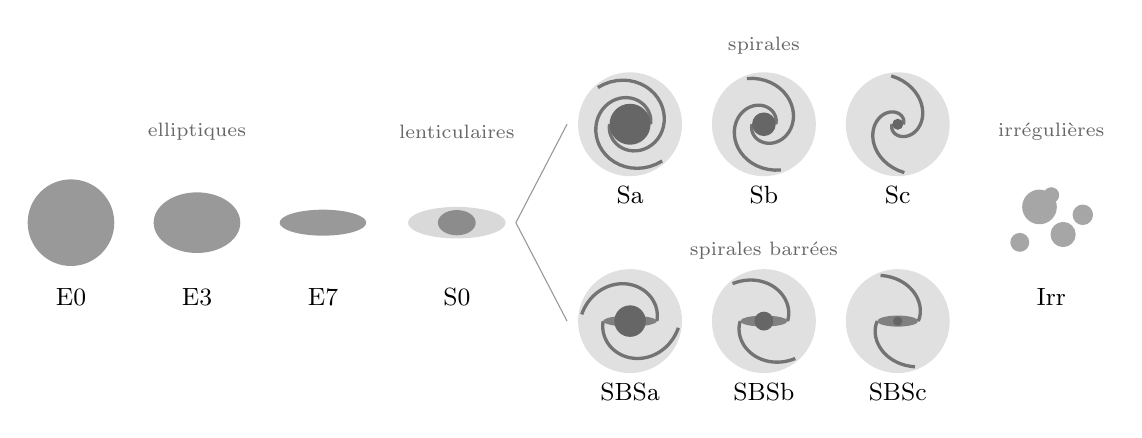
\begin{tikzpicture}[font=\small]
\def\spiralgal#1#2#3#4#5{% x, y, bulge radius, winding rate, bar half-length
  \begin{scope}[shift={(#1,#2)}]
    \fill[black!12] (0,0) circle (0.66);
    \pgfmathsetmacro{\rs}{max(#3,#5)}
    \pgfmathsetmacro{\th}{ln(0.62/\rs)/#4}
    \foreach \a in {0,180}
      \draw[line width=1.2pt, black!55, rotate=\a]
        plot[domain=0:\th, samples=40] ({\rs*exp(#4*\x)*cos(\x r)}, {\rs*exp(#4*\x)*sin(\x r)});
    \ifdim #5pt>0pt \fill[black!50] (0,0) ellipse (#5 and 0.07); \fi
    \fill[black!60] (0,0) circle (#3);
  \end{scope}}
\fill[black!40] (0,0) circle (0.55);
\fill[black!40] (1.6,0) ellipse (0.55 and 0.385);
\fill[black!40] (3.2,0) ellipse (0.55 and 0.165);
\fill[black!15] (4.9,0) ellipse (0.62 and 0.20);
\fill[black!45] (4.9,0) ellipse (0.24 and 0.16);
\draw[black!40] (5.65,0) -- (6.3,1.25);
\draw[black!40] (5.65,0) -- (6.3,-1.25);
\spiralgal{7.1}{1.25}{0.26}{0.16}{0}
\spiralgal{8.8}{1.25}{0.15}{0.28}{0}
\spiralgal{10.5}{1.25}{0.07}{0.45}{0}
\spiralgal{7.1}{-1.25}{0.20}{0.20}{0.34}
\spiralgal{8.8}{-1.25}{0.12}{0.32}{0.30}
\spiralgal{10.5}{-1.25}{0.06}{0.45}{0.26}
\foreach \p/\r in {(12.3,0.2)/0.22,(12.6,-0.15)/0.16,(12.05,-0.25)/0.12,(12.45,0.35)/0.1,(12.85,0.1)/0.13}
  \fill[black!35] \p circle (\r);
\foreach \x/\t in {0/E0,1.6/E3,3.2/E7,4.9/S0}
  \node at (\x,-0.95) {\t};
\foreach \x/\t in {7.1/Sa,8.8/Sb,10.5/Sc}
  { \node at (\x,0.35) {\t}; \node at (\x,-2.15) {SB\t}; }
\node at (12.45,-0.95) {Irr};
\node[font=\scriptsize, black!60] at (1.6,1.15) {elliptiques};
\node[font=\scriptsize, black!60] at (4.9,1.15) {lenticulaires};
\node[font=\scriptsize, black!60] at (8.8,2.25) {spirales};
\node[font=\scriptsize, black!60] at (8.8,-0.35) {spirales barrées};
\node[font=\scriptsize, black!60] at (12.45,1.15) {irrégulières};
\end{tikzpicture}
\par\smallskip{\small La \omterm{def:b3:milky-way-galaxies:types}{séquence de Hubble} représentée en forme de diapason,
de manière schématique. Les elliptiques sont notées d'après leur aplatissement
apparent~; le diapason se divise au niveau des lenticulaires en spirales ordinaires et spirales barrées,
ordonnées des grands bulbes et des bras très serrés (a) aux petits bulbes et
aux bras ouverts (c)~; les irrégulières ferment la séquence.}\label{fig:b3:milky-way-galaxies:fork}
\end{omfigure}
% ledger: buta11:hubble

Les classes décrivent des formes observées sur le ciel, et une même étiquette masque
une gamme~: une elliptique vue selon son axe le plus court paraît ronde, quel que soit
son aplatissement réel, et les frontières entre classes voisines relèvent
du jugement. Dans un catalogue des galaxies proches de nous, la
Galaxie est classée S(B)bc, une spirale entre Sb et Sc avec une barre~; sa grande
voisine Andromède (M31) est une Sb, la galaxie du Triangle (M33) une Sc, et
les Grand et Petit Nuage de Magellan sont des irrégulières.
% ledger: buta11:hubble, mcconn12:local-group

\begin{omfigure}
\centering
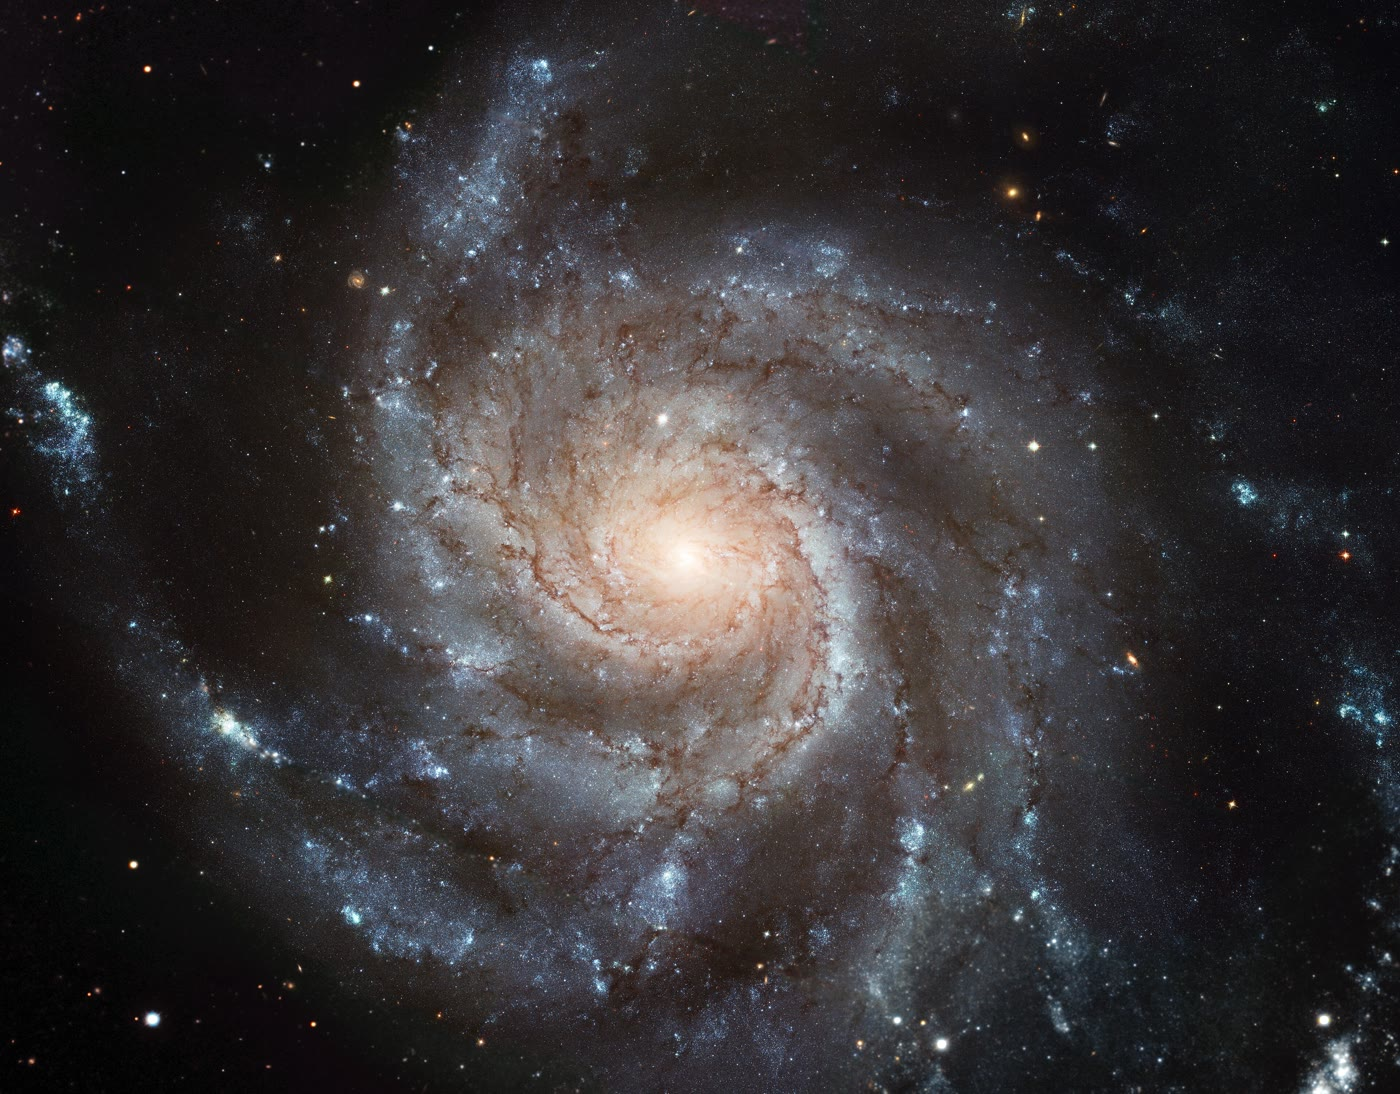
\includegraphics[width=0.66\linewidth]{images/book5/b3-m101.jpg}
\par\smallskip{\small La \omterm{def:b3:milky-way-galaxies:types}{galaxie spirale} M101 vue de face par le télescope spatial
Hubble, une mosaïque de 51 expositions, recadrée sur ses bords~: un bulbe petit,
brillant, jaunâtre~; des bras ouverts, plus bleus et parsemés d'amas
d'étoiles jeunes~; des traînées brunes de poussière le long des bras. Image ESA et NASA
(Hubble, heic0602), CC BY~4.0.}\label{fig:b3:milky-way-galaxies:m101}
\end{omfigure}
% ledger: photo:b3-m101

Pourquoi les bras spiraux ne s'enroulent-ils pas~? Dans un disque dont la \omterm{def:b3:milky-way-galaxies:rotation-curve}{courbe de rotation} est plate,
une étoile située à la moitié de la distance au centre fait un tour en moitié moins de temps.
Une spirale d'étoiles se resserrerait à chaque tour, et au bout de quelques tours
du disque elle deviendrait une bobine serrée (\cref{exo:b3:milky-way-galaxies:11}).

\begin{definition}[Théorie des ondes de densité]\label{def:b3:milky-way-galaxies:density-wave}
La \emph{théorie des ondes de densité}\index{théorie des ondes de densité} explique les bras spiraux
comme une onde de densité plus élevée dans un disque, un motif spiral qui tourne
d'un bloc à sa propre vitesse angulaire, la vitesse du motif, tandis que les étoiles et
le gaz le traversent, ralentissant en entrant dans le bras encombré et accélérant
à la sortie, comme des voitures qui traversent un embouteillage.
\end{definition}

La théorie, proposée en 1964, libère les bras du problème de l'enroulement.
Le gaz qui entre dans un bras est comprimé, et des étoiles s'y forment~: les bras
sont mis en évidence par les étoiles jeunes et le gaz lumineux, tandis que les vieilles étoiles sont
réparties beaucoup plus uniformément. Le caractère durable des bras en tant qu'ondes reste débattu~;
les simulations numériques de disques font plus souvent apparaître des bras transitoires,
qui se dissolvent et se reforment, et une galaxie voisine ou une barre peut entraîner
une spirale à deux bras.
% ledger: dobbs14:density-wave

\begin{definition}[Trou noir supermassif]\label{def:b3:milky-way-galaxies:smbh}
Un \emph{trou noir supermassif}\index{trou noir supermassif} est un trou noir
d'au moins un million de masses solaires, situé au centre d'une galaxie.
\end{definition}

Au centre de la Galaxie, la source radio compacte Sagittarius~A*
(Sgr~A*) se trouve parmi des étoiles en orbites serrées et rapides. Leurs orbites exigent une
masse centrale d'environ quatre millions de soleils, $\num[separate-uncertainty=true]{4.2 \pm 0.2 e6}$
masses solaires dans une synthèse des mesures. Sgr~A* bouge à peine
par rapport aux galaxies lointaines~: une fois le mouvement du Soleil retiré, son
mouvement résiduel ne dépasse pas quelques kilomètres par seconde, de sorte qu'il renferme
au moins un quart de cette masse. Sa taille est comparable à son rayon de Schwarzschild,
et sa densité, supérieure à \num{4e23} masses solaires par
parsec cube, est très proche de celle attendue pour un trou noir~: les indices
en faveur de la nature de trou noir de Sgr~A* sont écrasants.
% ledger: reid20:sgra, bhg16:structure, gravity19:r0

\begin{definition}[Groupe local~; amas de galaxies]\label{def:b3:milky-way-galaxies:groups}
Le \emph{Groupe local}\index{Groupe local} est le groupe de galaxies lié par la gravitation,
dominé par la Voie lactée et Andromède, chacune accompagnée de ses galaxies satellites.
Un \emph{amas de galaxies}\index{amas de galaxies} est l'un des plus grands
systèmes liés par la gravitation~: de nombreuses galaxies retenues, avec un gaz chaud
qui émet des rayons X, dans un puits commun constitué principalement de matière
noire.
\end{definition}

Plus d'une centaine de galaxies se trouvent à moins de \qty{3}{Mpc} du Soleil, pour la plupart
des naines. Le Grand Nuage de Magellan est à environ \qty{50}{kpc}, Andromède à
\qty{783}{kpc} et se rapproche de nous à \qty{300}{km.s^{-1}}, et les membres
liés du groupe se trouvent à environ \qty{1.06}{Mpc} de son centre de
masse, entre la Galaxie et Andromède, là où ils s'écartent de
l'expansion de l'Univers. Sa masse, déduite du mouvement des deux grandes
galaxies l'une vers l'autre, est de l'ordre de \num{5e12} masses solaires. Dans un
\omterm{def:b3:milky-way-galaxies:groups}{amas de galaxies} massif, le gaz chaud, à environ \qty{e8}{K}, représente environ dix
fois la masse des étoiles~; galaxies et gaz réunis sont trop légers pour
la profondeur du puits gravitationnel, et l'essentiel de la masse de l'amas,
de l'ordre de \num{e15} masses solaires, est sombre.
% ledger: mcconn12:local-group, kravtsov12:clusters

\section{L'échelle des distances}\label{sec:b3:milky-way-galaxies:ladder}

Une parallaxe donne une distance par la seule géométrie, mais les parallaxes diminuent
avec la distance. Le meilleur catalogue de parallaxes mesure une parallaxe avec une
incertitude de 0.02 à \qty{0.03}{mas} pour les étoiles plus brillantes que la
magnitude~15, ce qui donne une distance à \qty{10}{\percent} près jusqu'à environ
\qty{4}{kpc}~; le Grand Nuage de Magellan, à \qty{50}{kpc}, a une
parallaxe de \qty{0.02}{mas}. Au-delà, les distances reposent sur des objets dont la
luminosité est connue.
% ledger: gaia:dr3, freedman19:trgb

\begin{definition}[Chandelle standard~; échelle des distances]\label{def:b3:milky-way-galaxies:ladder}
Une \emph{chandelle standard}\index{chandelle standard} est une classe d'objets
dont la magnitude absolue est connue, ou peut être déduite d'une propriété
mesurée indépendamment de la distance, de sorte que sa magnitude apparente donne
son module de distance. L'\emph{échelle des distances}\index{échelle des distances} est
la chaîne de méthodes, chacune étalonnée sur des objets assez proches pour être
mesurés aussi par la méthode précédente, qui conduit des parallaxes jusqu'à
l'Univers en expansion.
\end{definition}

\begin{definition}[Céphéide~; loi de Leavitt]\label{def:b3:milky-way-galaxies:cepheid}
Une \emph{céphéide}\index{céphéide} est une étoile jeune, lumineuse et pulsante,
dont la luminosité varie avec une période rigoureusement régulière,
de environ un jour à plusieurs semaines. La \emph{loi de Leavitt}\index{loi de Leavitt},
ou relation période--luminosité, est la relation linéaire entre la magnitude
absolue moyenne d'une céphéide et le logarithme de sa période, les étoiles les
plus brillantes ayant des périodes plus longues.
\end{definition}

La relation a été découverte dans le Petit Nuage de Magellan, dont les étoiles
sont toutes à peu près à la même distance, en 1908. La poussière présente dans la galaxie qui
abrite une \omterm{def:b3:milky-way-galaxies:cepheid}{céphéide} l'assombrit et la rougit~; mais l'assombrissement est plus fort
dans le visible que dans le proche infrarouge, dans un rapport fixe pour un type donné de
poussière, et la combinaison $W_I = I - 1.55\,(V - I)$ des magnitudes dans
les bandes I et V, l'indice de Wesenheit, est choisie pour que l'assombrissement
s'annule. La figure ci-dessous le montre pour 2315 \omterm{def:b3:milky-way-galaxies:cepheid}{céphéides} du Grand Nuage de Magellan~: la \omterm{def:b3:milky-way-galaxies:cepheid}{loi de
Leavitt} est une droite serrée, avec une dispersion de
\qty{0.078}{mag}, soit \qty{3.6}{\percent} en distance pour une seule
étoile.
% ledger: sos15:leavitt, data:b5-ogle-lmc-cep

\begin{omfigure}
\centering
\begin{tikzpicture}
\begin{axis}[width=0.80\linewidth, height=0.52\linewidth,
  xmin=-0.05, xmax=1.6, ymin=10, ymax=16.6, y dir=reverse,
  xlabel={$\log_{10}(P/\mathrm{d})$}, ylabel={Indice de Wesenheit $W_I$ (mag)},
  tick label style={font=\scriptsize}, label style={font=\small},
  legend style={font=\scriptsize, at={(0.5,-0.17)}, anchor=north, legend columns=3, draw=none, cells={anchor=west}, /tikz/every even column/.append style={column sep=1em}},
  legend image post style={scale=2.2}]
\addplot[only marks, mark=*, mark size=0.45pt, omDef, opacity=0.6] table[x=logp, y=w] {figdata/out/bachelor-3-distance_ladder-pl.dat};
\addlegendentry{Céphéides}
\addplot[only marks, mark=x, mark size=1.6pt, red!70!black] table[x=logp, y=w] {figdata/out/bachelor-3-distance_ladder-clipped.dat};
\addlegendentry{écartées ($>3\sigma$)}
\addplot[thick, black] table[x=logp, y=w_fit] {figdata/out/bachelor-3-distance_ladder-fit.dat};
\addlegendentry{ajustement}
\node[font=\scriptsize, anchor=south west, fill=white, inner sep=1pt] at (axis cs:0.55,11.0) {$W_I = -3.315\log_{10}P + 15.889$};
\end{axis}
\end{tikzpicture}
\par\smallskip{\small La \omterm{def:b3:milky-way-galaxies:cepheid}{loi de Leavitt} dans le Grand Nuage de Magellan~:
l'indice de Wesenheit de 2315 \omterm{def:b3:milky-way-galaxies:cepheid}{céphéides} pulsant sur leur mode fondamental
en fonction du logarithme de leur période (relevé OGLE, Soszy\'nski et
al., 2015, via le CDS). Les étoiles les plus brillantes sont les plus hautes. Une droite
ajustée par moindres carrés, après avoir écarté 92 étoiles situées à plus de
trois écarts-types de celle-ci, reproduit la relation publiée
($-3.314$, $15.888$). Avec le module de distance du Nuage, 18.477, la droite
donne la magnitude absolue de Wesenheit de toute \omterm{def:b3:milky-way-galaxies:cepheid}{céphéide} à partir de sa période.}\label{fig:b3:milky-way-galaxies:leavitt}
\end{omfigure}
% ledger: data:b5-ogle-lmc-cep, sos15:leavitt, freedman19:trgb

\begin{definition}[Sommet de la branche des géantes rouges]\label{def:b3:milky-way-galaxies:trgb}
Le \emph{sommet de la branche des géantes rouges}\index{sommet de la branche des géantes rouges}
(TRGB) est la limite supérieure nette des luminosités des géantes rouges d'une
\omterm{def:b3:milky-way-galaxies:populations}{population stellaire} ancienne, fixée par l'allumage de l'hélium dans leur cœur,
le flash de l'hélium~; dans la bande I, elle se situe à peu près à la même
magnitude absolue dans toute population ancienne, $M_I \approx -4.05$ pour une
couleur $V - I = 1.6$, et ne dépend que faiblement de la composition chimique.
\end{definition}

Le sommet se mesure dans les halos peu denses des galaxies, où il y a peu de
poussière et peu d'encombrement~; il utilise de vieilles étoiles du halo là où
les \omterm{def:b3:milky-way-galaxies:cepheid}{céphéides} utilisent de jeunes étoiles du disque, et les deux méthodes n'ont aucune physique en commun. Le
TRGB et les \omterm{def:b3:milky-way-galaxies:cepheid}{céphéides} atteignent quelques dizaines de mégaparsecs, vers des galaxies où a explosé une
\omterm{def:b3:milky-way-galaxies:ladder}{chandelle standard} rare et bien plus brillante~: une supernova de type~Ia, l'explosion
thermonucléaire d'une naine blanche rappelée des volumes de physique,
dont la magnitude absolue au maximum, une fois corrigée de la
forme de sa courbe de lumière et de sa couleur, vaut
$M_B = \qty[separate-uncertainty=true]{-19.253 \pm 0.027}{mag}$. De telles
supernovae sont observées à travers des centaines de mégaparsecs.
% ledger: freedman19:trgb, riess22:h0

\begin{definition}[Relation de Tully--Fisher]\label{def:b3:milky-way-galaxies:tully-fisher}
La \emph{relation de Tully--Fisher}\index{relation de Tully--Fisher} est la
corrélation entre la luminosité, ou mieux la masse des étoiles et du gaz,
d'une \omterm{def:b3:milky-way-galaxies:types}{galaxie spirale} et la vitesse de sa \omterm{def:b3:milky-way-galaxies:rotation-curve}{courbe de rotation} plate~; sous sa
forme baryonique, $M_\mathrm{b} = A\,V^4$, elle vaut d'environ 30 à
\qty{300}{km.s^{-1}}.
\end{definition}

Le spectre à 21~cm d'une galaxie donne sa vitesse de rotation maximale, la
relation sa luminosité, indépendamment de sa distance, et son flux
donne alors la distance~: un barreau de l'échelle pour les \omterm{def:b3:milky-way-galaxies:types}{galaxies spirales} trop
lointaines pour les étoiles isolées. La Galaxie, par sa luminosité et sa rotation, se place sur la relation.
% ledger: mcgaugh00:btf, nrao:hi-line, bhg16:structure

\begin{omfigure}
\centering
\pgfplotstableread{figdata/out/bachelor-3-distance_ladder-ladder.dat}\laddertab
\pgfplotstableread{figdata/out/bachelor-3-distance_ladder-anchors.dat}\anchortab
\pgfplotstablegetelem{0}{d_hi}\of{\laddertab}\let\plxhi\pgfplotsretval
\pgfplotstablegetelem{1}{d_lo}\of{\laddertab}\let\cephlo\pgfplotsretval
\pgfplotstablegetelem{1}{d_hi}\of{\laddertab}\let\cephhi\pgfplotsretval
\pgfplotstablegetelem{3}{d_lo}\of{\laddertab}\let\snlo\pgfplotsretval
\pgfplotstablegetelem{3}{d_hi}\of{\laddertab}\let\snhi\pgfplotsretval
\pgfplotstablegetelem{1}{d}\of{\anchortab}\let\mthirtyone\pgfplotsretval
\pgfplotstablegetelem{2}{d}\of{\anchortab}\let\nfourtwo\pgfplotsretval
\begin{tikzpicture}
\begin{axis}[width=0.92\linewidth, height=0.42\linewidth,
  xmode=log, xmin=1e-3, xmax=2e6, ymin=0.4, ymax=4.9,
  ytick={1,2,3,4}, yticklabels={parallaxes, céphéides, TRGB, SN~Ia},
  xtick={1e-3,1e-2,1e-1,1,10,100,1e3,1e4,1e5,1e6},
  xticklabels={1\,pc,,,1\,kpc,,,1\,Mpc,,,1\,Gpc},
  xlabel={distance}, tick label style={font=\scriptsize}, label style={font=\small},
  y tick label style={font=\small}, axis y line*=left, axis x line*=bottom]
\draw[line width=7pt, omDef!70] (axis cs:1e-3,1) -- (axis cs:\plxhi,1);
\draw[line width=7pt, omMeth!70] (axis cs:\cephlo,2) -- (axis cs:\cephhi,2);
\draw[line width=7pt, omProp!70] (axis cs:\cephlo,3) -- (axis cs:\cephhi,3);
\draw[line width=7pt, red!60] (axis cs:\snlo,4) -- (axis cs:\snhi,4);
\draw[densely dotted, thick] (axis cs:\cephlo,0.4) -- (axis cs:\cephlo,4.55) node[anchor=south, font=\scriptsize] {LMC};
\draw[densely dotted, thick] (axis cs:\mthirtyone,0.4) -- (axis cs:\mthirtyone,4.55) node[anchor=south, font=\scriptsize] {M31};
\draw[densely dotted, thick] (axis cs:\nfourtwo,0.4) -- (axis cs:\nfourtwo,4.55) node[anchor=south, font=\scriptsize] {NGC~4258};
\draw[->, thick, black!60] (axis cs:\plxhi,1.25) to[out=30, in=200] (axis cs:\cephlo,1.75);
\draw[->, thick, black!60] (axis cs:\cephhi,2.25) to[out=40, in=220] (axis cs:\snlo,3.75);
\end{axis}
\end{tikzpicture}
\par\smallskip{\small Les barreaux de l'\omterm{def:b3:milky-way-galaxies:ladder}{échelle des distances}, avec les
distances sur lesquelles chacune est utilisée ici~: parallaxes du meilleur catalogue,
jusqu'à \qty{10}{\percent} jusqu'à \qty{4}{kpc}~; \omterm{def:b3:milky-way-galaxies:cepheid}{céphéides} et TRGB depuis le
Grand Nuage de Magellan jusqu'aux hôtes des supernovae de type~Ia les plus proches,
\qty{45}{Mpc}~; les supernovae de l'expansion régulière, pour des décalages vers
le rouge de 0.023 à 0.15 (\qtyrange{96}{616}{Mpc} pour $H_0 = 73$). Pointillés~:
deux ancrages de l'échelle des \omterm{def:b3:milky-way-galaxies:cepheid}{céphéides} à distances géométriques (binaires à
éclipses du Grand Nuage, masers à eau en orbite autour du trou noir de NGC~4258), et M31, la
plus proche grande spirale. Flèches~: chaque barreau est calibré sur des objets que le
barreau inférieur mesure aussi, les \omterm{def:b3:milky-way-galaxies:cepheid}{céphéides} de la Galaxie par leurs parallaxes,
les supernovae des galaxies proches par les \omterm{def:b3:milky-way-galaxies:cepheid}{céphéides} et le TRGB de leurs
hôtes.}\label{fig:b3:milky-way-galaxies:ladder-rungs}
\end{omfigure}
% ledger: gaia:dr3, riess22:h0, freedman19:trgb, mcconn12:local-group

Au sommet de l'échelle, les supernovae mesurent l'expansion de
l'Univers. La loi de Hubble, rappelée des volumes de physique, fait de la
vitesse de récession $cz$ d'une galaxie lointaine une grandeur proportionnelle à sa distance $d$,
$cz = H_0 d$ pour de petits décalages vers le rouge $z$~; la constante de Hubble $H_0$ est la
pente, et les supernovae, avec leurs distances issues de l'échelle, la donnent.

\begin{definition}[Tension de Hubble]\label{def:b3:milky-way-galaxies:tension}
La \emph{tension de Hubble}\index{tension de Hubble} est le désaccord entre la
valeur de la constante de Hubble mesurée localement avec l'\omterm{def:b3:milky-way-galaxies:ladder}{échelle des distances}
et la valeur déduite du rayonnement de fond diffus cosmologique
dans le modèle cosmologique standard.
\end{definition}

\begin{dated}{2022}
Les \omterm{def:b3:milky-way-galaxies:cepheid}{céphéides} des hôtes de 42 supernovae de type~Ia, ancrées sur les
parallaxes de Gaia, les masers de NGC~4258 et les binaires à éclipses du
Grand Nuage de Magellan, donnent
$H_0 = \qty[separate-uncertainty=true]{73.04 \pm 1.04}{km.s^{-1}.Mpc^{-1}}$.
Le \omterm{def:b3:milky-way-galaxies:trgb}{sommet de la branche des géantes rouges}, calibrant une centaine de
supernovae, donnait en 2019 $H_0 = 69.8 \pm 0.8 \pm \qty{1.7}{km.s^{-1}.Mpc^{-1}}$
(statistique et systématique). La carte du fond diffus cosmologique du satellite
Planck, lue avec le modèle cosmologique standard, implique
$H_0 = \qty[separate-uncertainty=true]{67.4 \pm 0.5}{km.s^{-1}.Mpc^{-1}}$.
La valeur \omterm{def:b3:milky-way-galaxies:cepheid}{céphéide} et la valeur du fond diffus diffèrent de cinq écarts-types~;
la valeur du TRGB se situe entre les deux. L'origine du
désaccord n'est pas connue~: une erreur non encore trouvée dans l'un des échelons,
ou une physique absente du modèle.
\end{dated}
% ledger: riess22:h0, freedman19:trgb, planck18:h0

\begin{inthelab}[Un satellite astrométrique et son catalogue]
Le satellite Gaia balaie le ciel selon un parcours programmé, de sorte que chaque
étoile est mesurée encore et encore au cours de la mission. Au sol, les
unités de coordination d'un consortium de traitement des données transforment ces
mesures en une position, une parallaxe et un mouvement propre pour chacune des
plus d'un milliard de sources~: des petits mouvements apparents d'une étoile sur la voûte céleste,
la parallaxe est la part qui se répète chaque année, et le mouvement propre
la part qui s'accumule. Chaque catalogue est publié avec des articles qui
décrivent son traitement et sa validation, et chaque distance des
figures de cette section qui repose sur une parallaxe repose sur un tel
catalogue.
\end{inthelab}

\begin{dated}{2022}
Le troisième catalogue Gaia, publié le 13 juin 2022 à partir de 34 mois de
observations, donne les positions, les parallaxes et les mouvements propres de près de
1.46~milliard de sources, de la magnitude~3 à~21, et les vitesses radiales moyennes
de 33~millions d'étoiles. Ses incertitudes sur la parallaxe valent 0.02 à
\qty{0.03}{mas} pour les étoiles plus brillantes que la magnitude~15, \qty{0.07}{mas} à
la magnitude~17, et \qty{0.5}{mas} à la magnitude~20.
\end{dated}
% ledger: gaia:dr3

\section{Exercices}

\begin{exercise}[$\star$]\label{exo:b3:milky-way-galaxies:1}
L'année galactique du Soleil. (a)~Avec $R_0 = \qty{8.178}{kpc}$ et
$V_0 = \qty{229}{km.s^{-1}}$, calculer la période de l'orbite du Soleil
autour du centre galactique, en millions d'années. (b)~Combien de tours le Soleil a-t-il
effectués depuis la formation du Système solaire, il y a \qty{4.54}{Ga}~?
\end{exercise}

\begin{exercise}[$\star$]\label{exo:b3:milky-way-galaxies:2}
Le mouvement de réaction de Sgr~A*. (a)~Un mouvement propre de \qty{1}{mas} par an
à \qty{1}{kpc} correspond à une vitesse transverse de \qty{1}{au} par an~: exprimer cette vitesse en
kilomètres par seconde. (b)~Sgr~A*, supposé au repos au centre galactique
à \qty{8.178}{kpc}, dérive le long du plan galactique de \qty{6.411}{mas}
par an. Calculer la vitesse du Soleil autour du centre et la comparer à la
valeur de référence, \qty[separate-uncertainty=true]{248 \pm 3}{km.s^{-1}}. (c)~Retrancher le
mouvement particulier du Soleil dans le sens de rotation, \qty{11}{km.s^{-1}}, et
comparer avec $V_0$ issu de la \omterm{def:b3:milky-way-galaxies:rotation-curve}{courbe de rotation}.
\end{exercise}

\begin{exercise}[$\star$]\label{exo:b3:milky-way-galaxies:3}
Classification des elliptiques. (a)~Les isophotes d'une \omterm{def:b3:milky-way-galaxies:types}{galaxie elliptique} ont un
rapport d'axes de 0.6~: donner sa classe. (b)~Quel rapport d'axes possède une E7~?
(c)~Pourquoi une galaxie E0 peut-elle être un système aplati~?
\end{exercise}

\begin{exercise}[$\star$]\label{exo:b3:milky-way-galaxies:4}
Calibrateurs. Calculer les distances du Grand Nuage de Magellan
($\mu = 18.477$), d'Andromède ($\mu = 24.47$) et NGC~4258
($\mu = 29.398$). Quelle parallaxe aurait une étoile du Nuage, et pourquoi
la distance du Nuage ne peut-elle pas être mesurée par parallaxes~?
\end{exercise}

\begin{exercise}[$\star\star$]\label{exo:b3:milky-way-galaxies:5}
À partir des \omterm{def:b3:milky-way-galaxies:rotation-curve}{constantes d'Oort} $A = \qty{15.3}{km.s^{-1}.kpc^{-1}}$ et
$B = \qty{-11.9}{km.s^{-1}.kpc^{-1}}$~: (a)~calculer la vitesse angulaire du
\omterm{def:b3:milky-way-galaxies:lsr}{référentiel local au repos} et, avec $R_0 = \qty{8.178}{kpc}$, la vitesse circulaire $V_0$~;
(b)~calculer la pente de la \omterm{def:b3:milky-way-galaxies:rotation-curve}{courbe de rotation} au niveau du Soleil. (c)~Comparer
à la \omterm{def:b3:milky-way-galaxies:rotation-curve}{courbe de rotation} des géantes rouges ($V_0 = \qty{229.0}{km.s^{-1}}$,
de pente \qty{-1.7}{km.s^{-1}} par kiloparsec) et proposer pourquoi les deux
diffèrent, sachant que la même mesure trouve $C$ et $K$ non nuls.
\end{exercise}

\begin{exercise}[$\star\star$]\label{exo:b3:milky-way-galaxies:6}
\omterm{def:b3:milky-way-galaxies:rotation-curve}{Courbe de rotation} plate et densité locale. (a)~Pour une galaxie sphérique
dont la \omterm{def:b3:milky-way-galaxies:rotation-curve}{courbe de rotation} est plate à \qty{229}{km.s^{-1}}, calculer la densité à
\qty{8.178}{kpc}, en masses solaires par parsec cube
($G = \qty{4.301e-6}{kpc.(km.s^{-1})^2}$ par masse solaire). (b)~Montrer que
une masse solaire par parsec cube vaut \qty{37.96}{GeV.cm^{-3}}, et exprimer
la densité locale de matière noire, \qty{0.30}{GeV.cm^{-3}}, en masses solaires
par parsec cube. (c)~Pourquoi la densité de (a) est-elle plus élevée~?
\end{exercise}

\begin{exercise}[$\star\star$]\label{exo:b3:milky-way-galaxies:7}
Distance d'une \omterm{def:b3:milky-way-galaxies:cepheid}{céphéide}. Dans une \omterm{def:b3:milky-way-galaxies:types}{galaxie spirale} fictive, une \omterm{def:b3:milky-way-galaxies:cepheid}{céphéide} de période
\qty{30}{d} possède un indice de Wesenheit moyen $W_I = \qty{25.00}{mag}$.
(a)~En utilisant la \omterm{def:b3:milky-way-galaxies:cepheid}{loi de Leavitt} du Grand Nuage de Magellan,
$W_I = -3.314\log_{10}P + 15.888$, et le module de distance du Nuage
18.477, calculer la magnitude absolue de Wesenheit de la \omterm{def:b3:milky-way-galaxies:cepheid}{céphéide}. (b)~Calculer
la distance de la galaxie. (c)~La dispersion de la loi est de \qty{0.077}{mag}~: quelle est
l'erreur relative sur la distance due à une seule \omterm{def:b3:milky-way-galaxies:cepheid}{céphéide}, et à cinquante~?
\end{exercise}

\begin{exercise}[$\star\star$]\label{exo:b3:milky-way-galaxies:8}
Distance TRGB. Dans le halo d'une galaxie fictive, le \omterm{def:b3:milky-way-galaxies:trgb}{sommet de la branche des
géantes rouges} est trouvé à $I = \qty{26.00}{mag}$~; la poussière le long de la ligne de
visée atténue la bande I de \qty{0.05}{mag}. Avec $M_I = -4.05$, calculer le module de
distance et la distance. Que signifie une incertitude de
\qty{0.04}{mag} sur le sommet en termes de distance~?
\end{exercise}

\begin{exercise}[$\star\star$]\label{exo:b3:milky-way-galaxies:9}
La constante de Hubble à partir des supernovae. Pour une supernova de l'expansion régulière,
$\log_{10}(cz) - 0.2\,m_B = a_B$, l'ordonnée à l'origine du
diagramme de Hubble des supernovae, et le module de distance est
$m_B - M_B = 5\log_{10}(d/\mathrm{Mpc}) + 25$. (a)~Montrer que
$\log_{10}H_0 = 0.2\,M_B + a_B + 5$ ($H_0$ en kilomètres par seconde et par
mégaparsec). (b)~Avec $M_B = -19.253$ et $a_B = 0.714158$, calculer $H_0$.
(c)~Quelle valeur de $M_B$ donnerait $H_0 = \qty{67.4}{km.s^{-1}.Mpc^{-1}}$~? De combien
de magnitudes, et de quelle fraction des distances, les deux
calibrations diffèrent~?
\end{exercise}

\begin{exercise}[$\star\star\star$]\label{exo:b3:milky-way-galaxies:10}
D'où vient la \omterm{def:b3:milky-way-galaxies:tully-fisher}{relation de Tully--Fisher}. (a)~Une galaxie à disque de masse $M$
de rayon $R$ tourne à $V$~: montrer que $M \approx RV^2/G$. (b)~Si toutes les
\omterm{def:b3:milky-way-galaxies:types}{galaxies spirales} avaient la même densité surfacique moyenne $\Sigma = M/(\pi R^2)$,
montrer que $M \propto V^4$. (c)~Deux galaxies fictives sur la même relation baryonique
tournent à 100 et \qty{229}{km.s^{-1}}~: quel est le rapport des
leurs masses~? (d)~Deux galaxies tournent à la même vitesse et ont la même
luminosité~; l'une reçoit quatre fois le flux de l'autre. Comparer leurs
distances.
\end{exercise}

\begin{exercise}[$\star\star\star$]\label{exo:b3:milky-way-galaxies:11}
Le problème de l'enroulement. Un disque tourne avec une courbe plate à
\qty{229}{km.s^{-1}}. (a)~Convertir cette vitesse en kiloparsecs par milliard
d'années. (b)~Un bras rectiligne d'étoiles s'étend à l'instant zéro de 4 à
\qty{12}{kpc}. Calculer les périodes orbitales aux deux extrémités. (c)~Après
\qty{1}{Ga}, de quel angle son extrémité intérieure a-t-elle pris de l'avance
sur son extrémité extérieure~? Combien de tours de spirale cela représente-t-il, et à quoi
ressemblerait le bras~? (d)~Comment une onde de densité évite-t-elle ce problème~?
\end{exercise}

\begin{exercise}[$\star\star\star$]\label{exo:b3:milky-way-galaxies:12}
Le trou noir au centre. Prendre pour masse centrale
\num{4.2e6} masses solaires et $R_0 = \qty{8178}{pc}$. (a)~L'étoile S2
tourne autour de lui en \num{16}~ans~: calculer le demi-grand axe de son orbite en
unités astronomiques (troisième loi de Kepler en unités solaires, $a^3 = MP^2$ avec
$a$ en au, $P$ en années et $M$ en masses solaires) ainsi que sa taille angulaire vue
depuis la Terre. (b)~Calculer le rayon de Schwarzschild du trou noir en
mètres et en unités astronomiques, ainsi que l'angle sous lequel son diamètre
est vu depuis la Terre, en microsecondes d'arc. (c)~Calculer la densité moyenne
de la masse contenue dans son rayon de Schwarzschild, en masses solaires par
parsec cube, et la comparer à la borne inférieure fixée par le mouvement de Sgr~A*,
\num{4e23} masses solaires par parsec cube.
\end{exercise}

\section{Problème~: peser la Galaxie}

\begin{problem}[{Problème du week-end --- à partir des mouvements des étoiles et du gaz jusqu'à
la matière noire à l'intérieur de \qty{20}{kpc}}]
\label{pb:b3:milky-way-galaxies:1}
Prendre $R_0 = \qty{8.18}{kpc}$, $G = \qty{4.301e-6}{kpc.(km.s^{-1})^2}$ par
masse solaire, et \qty{4.74}{km.s^{-1}} pour un mouvement propre de
\qty{1}{mas} par an à \qty{1}{kpc}. Toutes les vitesses sont relatives au
\omterm{def:b3:milky-way-galaxies:lsr}{référentiel local au repos}. Utiliser les théorèmes d'Oort et du point tangent du chapitre, et
l'approximation sphérique $M = RV^2/G$ pour les masses dynamiques.

\medskip\noindent\textbf{Partie I --- La rotation locale.} Un
relevé fictif d'étoiles de la bosse des géantes rouges, toutes à $d = \qty{1.00}{kpc}$ dans le
plan galactique, donne une vitesse radiale moyenne de \qty{+15.4}{km.s^{-1}} à
$\ell = \ang{45}$ et \qty{-15.2}{km.s^{-1}} à $\ell = \ang{135}$, et des
mouvements propres moyens en longitude de \qty{-5.91}{mas} par an à
$\ell = \ang{90}$ et \qty{+0.55}{mas} par an à $\ell = \ang{0}$.
\begin{enumerate}
\item Que prédit la formule d'Oort pour les vitesses radiales à
  $\ell = \ang{45}$, \ang{90}, \ang{135} et \ang{180}~?
\item Calculer $A$ à partir des deux vitesses radiales.
\item Calculer $B$ à partir du mouvement propre à $\ell = \ang{90}$.
\item Calculer à nouveau $B$ à partir du mouvement propre à $\ell = \ang{0}$, et
  comparer.
\item Calculer la vitesse angulaire du \omterm{def:b3:milky-way-galaxies:lsr}{référentiel local au repos} et la vitesse
  circulaire $V_0$.
\item Calculer la pente de la \omterm{def:b3:milky-way-galaxies:rotation-curve}{courbe de rotation} au Soleil. La courbe est-elle
  croissante, plate ou décroissante~?
\item Calculer la période de l'orbite du Soleil et le nombre de tours en
  \qty{4.54}{Ga}.
\end{enumerate}

\medskip\noindent\textbf{Partie II --- La courbe de rotation interne.} Prendre
$V_0 = \qty{229}{km.s^{-1}}$. Les vitesses radiales maximales des
profils à 21~cm à $\ell = \ang{40}$, \ang{50}, \ang{60} et \ang{70} sont
82.9, 55.6, 32.4 et \qty{14.9}{km.s^{-1}}.
\begin{enumerate}[resume]
\item Pourquoi la méthode du point tangent exige-t-elle $\ang{0} < \ell < \ang{90}$
  (ou le quadrant symétrique), et pourquoi échoue-t-elle au-delà du cercle solaire~?
\item Calculer le rayon du point tangent pour chaque longitude.
\item Calculer $V(R)$ en chaque point tangent.
\item De combien, en kilohertz, la raie du gaz au point tangent
  à $\ell = \ang{40}$ est-elle décalée par rapport à sa fréquence de repos,
  \qty{1420.405751}{MHz}, et dans quel sens~?
\item Comparer avec la courbe des géantes rouges, qui donne \qty{226.8}{km.s^{-1}}
  à \qty{5.27}{kpc} et \qty{229.6}{km.s^{-1}} à \qty{7.22}{kpc}. La courbe
  interne est-elle croissante, plate ou décroissante~?
\item Si la vitesse au point tangent à $\ell = \ang{40}$ était celle d'une
  masse ponctuelle au centre portant le Soleil à $V_0$, quelle serait-elle~?
  Que dit la comparaison de la répartition de la masse~?
\end{enumerate}

\medskip\noindent\textbf{Partie III --- La masse visible.} Utiliser le modèle de
masse du chapitre, en masses solaires et en kiloparsecs~: un
bulbe de Plummer $M = \num{1.067e10}$, $b = 0.3$~; un disque mince de Miyamoto--Nagai
$M = \num{3.944e10}$, $a = 5.3$, $b = 0.25$~; un \omterm{def:b3:milky-way-galaxies:structure}{disque épais} de même
masse avec $a = 2.6$, $b = 0.8$.
\begin{enumerate}[resume]
\item Calculer la masse visible totale du modèle et la comparer à la
  valeur de référence de la masse stellaire de la Galaxie, \qty[separate-uncertainty=true]{5 \pm 1 e10}{} masses
  solaires.
\item Calculer la vitesse circulaire du seul bulbe à \qty{20}{kpc}.
\item Calculer celles du disque mince et du \omterm{def:b3:milky-way-galaxies:structure}{disque épais} à \qty{20}{kpc}.
\item Calculer la vitesse circulaire de toute la masse visible à
  \qty{20}{kpc}.
\item Calculer la même chose à $R_0$, et comparer avec $V_0$.
\item Si toute la masse visible était concentrée au centre, quelle serait
  la vitesse à \qty{20}{kpc}~? Pourquoi la valeur du modèle en est-elle proche~?
\end{enumerate}

\medskip\noindent\textbf{Partie IV --- La matière noire.} Les géantes rouges
donnent une vitesse circulaire de \qty{200}{km.s^{-1}} à \qty{20}{kpc}.
\begin{enumerate}[resume]
\item Calculer la masse dynamique à l'intérieur de \qty{20}{kpc}.
\item Calculer la masse dynamique de la matière visible à l'intérieur de
  \qty{20}{kpc}.
\item Calculer la masse de matière noire à l'intérieur de \qty{20}{kpc}, et montrer que
  sa fraction vaut $1 - (V_\mathrm{vis}/V)^2$.
\item Le halo de NFW ajusté sur toute la courbe a
  $\rho_0 = \num{1.06e7}$ masses solaires par kiloparsec cube et
  $R_s = \qty{14.8}{kpc}$. Calculer sa masse à l'intérieur de \qty{20}{kpc} et la
  fraction sombre qu'elle implique. Pourquoi diffère-t-elle de la réponse précédente~?
\item Calculer la densité de ce halo en $R_0$, en masses solaires par
  parsec cube et en \unit{GeV.cm^{-3}} (une masse solaire par parsec cube
  vaut \qty{37.96}{GeV.cm^{-3}}).
\item Donner la fraction de matière noire dans la masse à l'intérieur de \qty{20}{kpc}
  déduite de la vitesse mesurée, en pour cent, à deux
  chiffres significatifs.
\end{enumerate}
\end{problem}
% ledger: gravity19:r0, eilers19:table1, pouliasis17:model1, eilers19:halo, bhg16:structure, nrao:hi-line, const:G, const:au, iau:parsec, usgs:age-earth
